%نام و نام خانوادگی:
%شماره دانشجویی: 
\مسئله{\lr{SDT}}

\پاسخ{
\begin{itemize}
\item
اگر آخر رشته - باشد می‌آید کمترین عدد مجموعه را حساب می‌کند و در صورتی که + باشد بیشترین عدد را در مجموعه محاسبه می‌کند.
\item
\lr{
‫‪synthesized‬‬ => \{S.val , A.val , Sign.sign\}
}
\newline
\lr{
inherited => \{Asign\}
}
\item
\begin{figure}
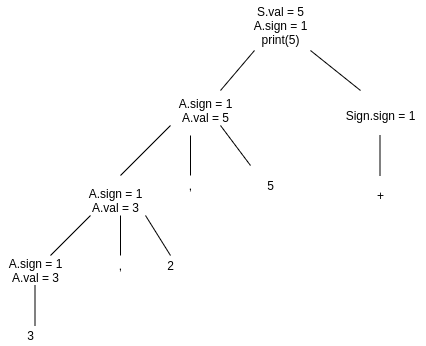
\includegraphics[width = \linewidth]{commons/Q2.png}
\end{figure}
\end{itemize}




}
